d
\documentclass[preprint,3p, 11pt,authoryear]{elsarticle}


\usepackage{graphicx}
\graphicspath{{./Graphic/}}
\usepackage{array}
\usepackage{amssymb} % various useful mathematical symbols
\usepackage{gensymb} % for `degree' sign
\usepackage{amsthm}  % extended theorem environments
\usepackage{lineno}   % for line numbers
\usepackage{tabularx} % for adjustable table width
\usepackage[hidelinks]{hyperref}  % for hyperlinks
\usepackage{amsmath}
\newtheorem{property}{Property}[section]
\usepackage{soul}
\usepackage{epsfig}
\usepackage{tabularx}
\usepackage{multirow} 
\usepackage{setspace}
\usepackage{adjustbox}
\usepackage{xcolor}


\journal{Nondestructive Testing and Evaluation}

\begin{document}

\begin{frontmatter}



\title{A methodology for calculating active source-time functions from broadband piezoelectric sensors in the laboratory}

 \author[1]{Paul A. Selvadurai \corref{cor1}}
 \ead{paul.selvadurai@sed.ethz.ch}
\author[2]{Rui Wu}
\author[3]{Claudio Madonna}




\cortext[cor1]{Corresponding author, Post-Doctoral fellow}
\address[1]{Swiss Seismological Service, ETH Zurich, Zurich, Switzerland}
\address[2]{Engineering Geology Group, ETH Zurich, Zurich, Switzerland}
\address[3]{Department of Earth Sciences, ETH Zurich, Zurich, Switzerland}



\begin{abstract}

\end{abstract}

\begin{keyword}
Acoustic emissions, absolutely calibrated sensors, active source time function, empirical Green's functions
\end{keyword}
\end{frontmatter}

\doublespacing
\linenumbers
\clearpage
%%%%%%%%%%%%%%%%%%%%%%%%%%%%%%%%%%%%%%%%%%%%%%%%%%%%%%%%%%%%%%%%%%%%%%%%%%%%%%%%%%%%%%%%%%%%%%%%%%%%%%%%%%%%%%%%%%%%%%%%%%%%%
\section{Introduction}
\label{int}



\section{Experimental facilities}
\subsection{General}

\begin{figure}[ht]
     	\centering
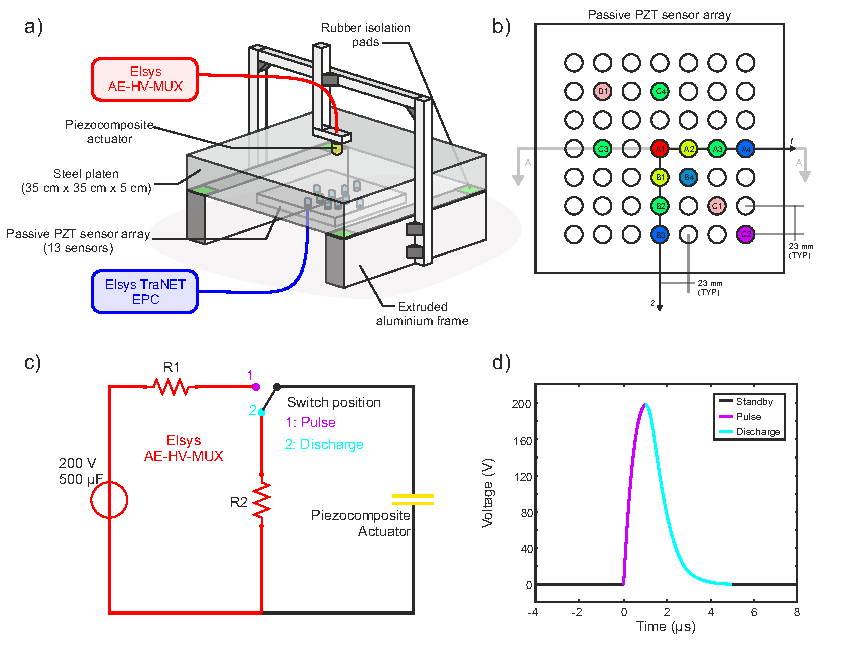
\includegraphics[scale= 1.0]{FIG1.pdf} 
\caption{\textbf{(a)}  }
	\label{fig1} 
\end{figure}

\begin{figure}[ht]
     	\centering
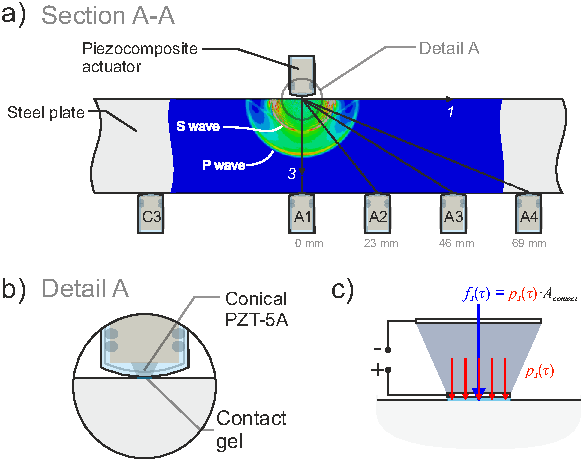
\includegraphics[scale= 1.0]{FIG2.pdf} 
\caption{\textbf{(a)}  }
	\label{fig2} 
\end{figure}

\subsection{Material properties}


\subsection{Elsys Instruments High-voltage Multiplexer}
***need information on \textbf{Piezosystem Jena HVP1000/100MODext.} from Roman Bertschi***



\section{Theory}
\label{theo}
We review the methodology that will model the forces produced by an active source piezoelectric transducer.  This methodology takes advantage of the theory surrounding elastodynamic wave propagation in an elastic medium.  We build on the recent studies of signal analysis and instrument calibration by \citet{McLaksey2012} continuing this analysis using Green's function formalization \citep{Aki2002, Johnson1974}. We assume that wave propagation can be adequately described by convolution with the Green's function and that each component in our analysis can be modeled as a linear-time invariant system.  We are assuming that changes in the sensor and source behavior and material properties are unaffected over time.  We assume point representations of both the sensor and source location. This so-called ``aperture'' effect is minimized by using the point contact conical PZT crystal but some deviations might be incurred.

Using the classical theory describing dynamic elasticity \citep{Aki2002}, we can use Green's functions to relate the displacement $u$ at a known location $\mathbf{x}$ and time $t$ to a force $f$ at another point $\mathbf{\xi}$ and time $\tau$, which is given as the convolution of the force with the Green's function

\begin{equation}
\label{eq1}
           u_{k}\left( \mathbf{x}, t \right)  =  
            f_{j}\left( \mathbf{\xi}, \tau \right) \ast 
            g_{kj}\left( \mathbf{x}, t;\mathbf{\xi}, \tau \right).
\end{equation}

\noindent We note that $\ast$ represents convolution in the time domain, $f$ is the force acting in the $j$ direction at location $\mathbf{\xi}$ and $g_{kj}\left( \mathbf{x}, t;\mathbf{\xi}, \tau \right)$ is the elastodynamic Green's function describing the displacement $u$ in the direction $k$ at location $\mathbf{x}$.  The true Green's function describes the displacement at time $t$ and location $\mathbf{x}$ for the unit impulse force at location $\mathbf{\xi}$ at the delayed time $\tau$. 

Piezoelectric transducers measure a voltage caused by the compression of the lead zirconate titanate (PZT) crystal in the surface normal direction $s\left( \mathbf{x}, t \right)$. We can relate the true surface displacement $u_{k}$ to voltage measurement $s$ using the instrument response, which is given as

    \begin{equation}
    \label{eq2}
        s\left( \mathbf{x}, t \right) =
            u_{k}\left( \mathbf{x}, t \right) \ast i_{k}\left(t \right).
    \end{equation}

\noindent Combining \eqref{eq1} and \eqref{eq2}, we can represent the measured voltage to the forces which produced them:

    \begin{equation}
    \label{eq3}
        s\left( \mathbf{x}, t \right) =
            u_{k}\left( \mathbf{x}, t \right) \ast i_{k}\left(t \right) =  
                f_{j}\left( \mathbf{\xi}, \tau \right) \ast 
                g_{kj}\left( \mathbf{x}, t;\mathbf{\xi}, \tau \right) \ast i_{k}\left( t \right).
    \end{equation}

\noindent We can also use this formulation to relate the measured signals to a set of self-equilibrating forces or moments $m_{jp}$ \citep{Aki2002}. Displacements in the body are related to the spatial derivative of the elastodynamic Green's function $g_{kj,p}$.  While this is more similar to sources buried within a specimen and may be more representative of an earthquake source, this is not the focus of this study.  In this study, all sources are produced on the surface of the specimen, which justifies the use of only equation \eqref{eq2}.

Our study aims at determining the nature of the source produced that occurs we use the PZT crystal as active source. WE first decompose the source into two parts as shown here:

\begin{equation}
    \label{eq4}
    f_{j}\left( \mathbf{\xi}, \tau \right) = f^{*}_{j}\left( \mathbf{\xi}, \tau \right)  \ast \kappa \left( \tau \right),
\end{equation}

\noindent where $f^{*}_{j}$ is the normalized force-time function that has units (N) and a general shape to that follows the electro-mechanical behavior of the coupled high-voltage discharge and sensor systems.  A unitless scaling factor $\kappa$ will be used to scale the normalized force time-function $f^{*}$ to the true force-time function $f$ and likely varies with the time as the electrical pulse is applied to the active source.

We use properties of the Fourier transform \citep{Bracewell1986} to help deconvolve equations \eqref{eq3} and \eqref{eq4}.  In the frequency domain, convolution and deconvolution simply becomes multiplication and division. This allows us to isolate the components of interest we wish to quantify for our analysis. An example of the instrument response in the frequency domain $I_{w}$ simplifies to:

\begin{equation}
    \label{eq5}
        I_{k}\left(\omega \right) = 
        S\left( \mathbf{x}, \omega \right) \cdot \left[ F_{j}\left( \mathbf{\xi}, \hat{\omega} \right) \cdot G_{kj}\left( \mathbf{x}, \omega; \mathbf{\xi}, \hat{\omega} \right)\right]^{-1} .
\end{equation}

\noindent where $I_{k}$, $S$, $F_{j}$ and $G_{kj}$ are calculated from the temporal Fourier transforms of the $i_{k}$, $s$, $f_{j}$ and $g_{kj}$, respectively.  As we will see in Section \ref{XXX}, instrument responses was calculated for the sensor array shown in Figure \ref{fig1}, where a controlled force-time function were applied at the central location by dropping small steel balls of different diameters onto the surface from a known height. According to Hertzian contact theory, it is possible to assume a source time function that is a function of the material properties of the ball and steel platen ($E, \nu, \rho$), the radius of ball, and the drop height. This method has been popularized over the recent years due to a highly reliable and repeatable force-time function $f$ produced from ball impact and the ability to absolutely calibrate the acoustic emission sensors over a wide spectral range \citep{McLaskey2010, McLaskey2012, McLaskey2015}.

We will use the known instrument response to better understand the source produced from the active PZT transducer.  We can rearrange equation \eqref{eq5} to obtain the true force in the frequency domain:

\begin{equation}
    \label{eq6}
\begin{split}
F_{j}\left( \mathbf{\xi}, \hat{\omega} \right) & = 
        S\left( \mathbf{x}, \omega \right) \cdot \left[ I_{k}\left(\omega \right) \cdot G_{kj}\left( \mathbf{x}, \omega; \mathbf{\xi}, \hat{\omega} \right)\right]^{-1}, \\
\end{split}
\end{equation}

\noindent where by combing the Fourier transform of equation \eqref{eq4} we obtain an expression for the normalized force-time function,

\begin{equation}
    \label{eq7}
\begin{split}
F^{*}_{j}\left( \mathbf{\xi}, \hat{\omega} \right) & = 
        S\left( \mathbf{x}, \omega \right) \cdot \left[ K\left(\hat{\omega}\right) \cdot I_{k}\left(\omega \right) \cdot G_{kj}\left( \mathbf{x}, \omega; \mathbf{\xi}, \hat{\omega} \right)\right]^{-1}.\\     
\end{split}
\end{equation}

\noindent To solve the features about $F^{*}_{j}$, we will need to \textit{a priori} knowledge of sensors instrument response, also needed will be signal measurements $S$ and the true Green's function $G_{kj}$ but we will still not know the frequency-dependent scaling function $K(\hat{\omega})$.




\begin{figure}[ht]
     	\centering
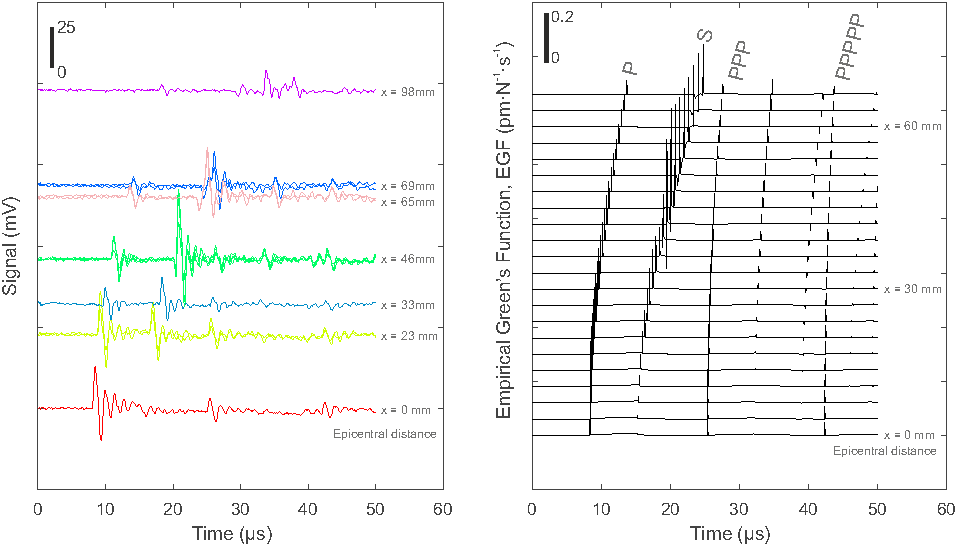
\includegraphics[scale= 1.0]{FIG3.pdf} 
\caption{\textbf{(a)}  }
	\label{fig3} 
\end{figure}

\begin{figure}[ht]
     	\centering
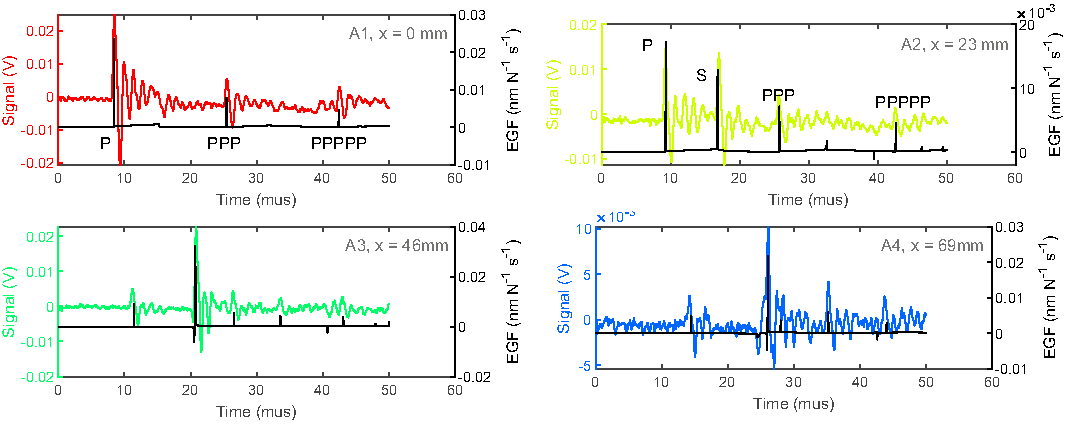
\includegraphics[scale= 0.90]{FIG4.pdf} 
\caption{\textbf{(a)}  }
	\label{fig4} 
\end{figure}

\begin{figure}[ht]
     	\centering
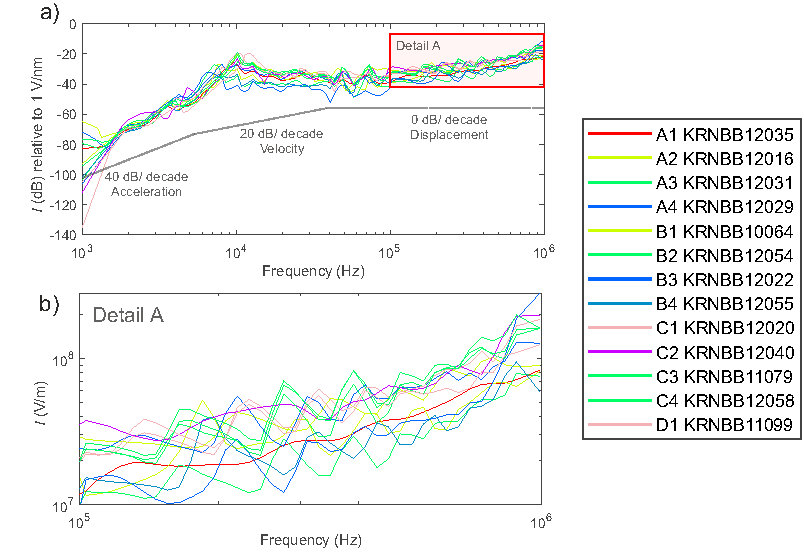
\includegraphics[scale= 0.9]{FIG5.pdf} 
\caption{\textbf{(a)}  }
	\label{fig5} 
\end{figure}


\begin{figure}[ht]
     	\centering
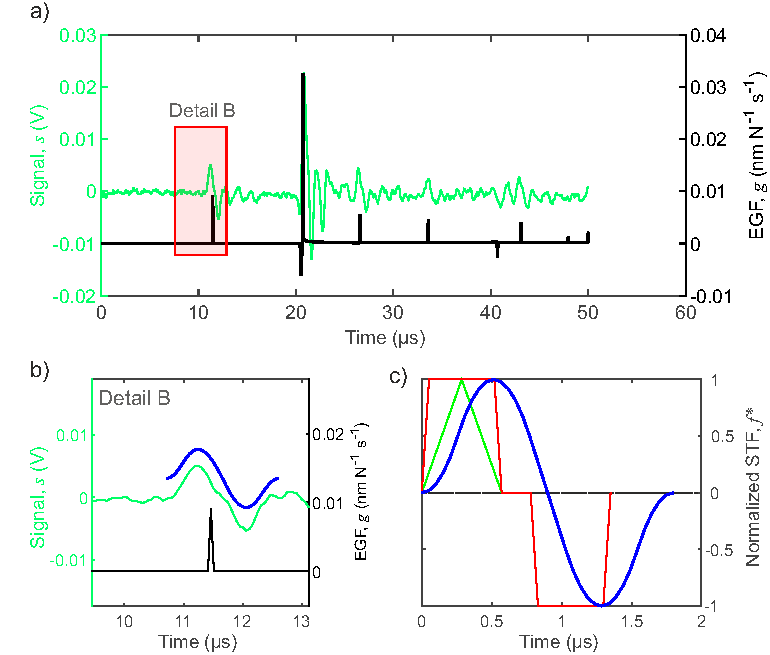
\includegraphics[scale= 0.9]{FIG6.pdf} 
\caption{\textbf{(a)}  }
	\label{fig6} 
\end{figure}


\begin{figure}[ht]
     	\centering
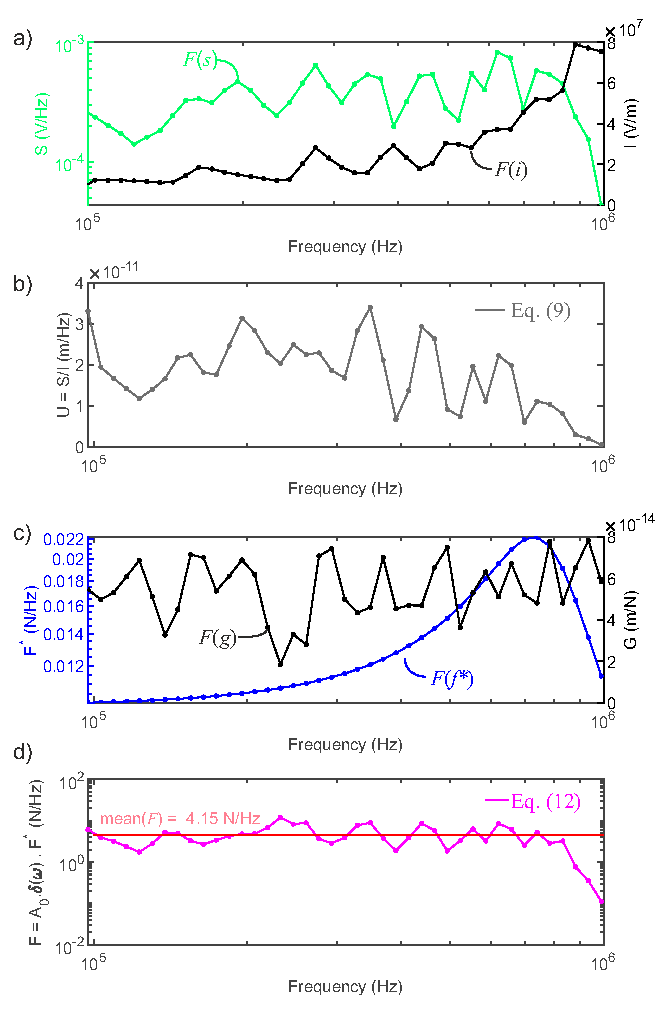
\includegraphics[scale= 1]{FIG7.pdf} 
\caption{\textbf{(a)}  }
	\label{fig7} 
\end{figure}


\begin{figure}[ht]
     	\centering
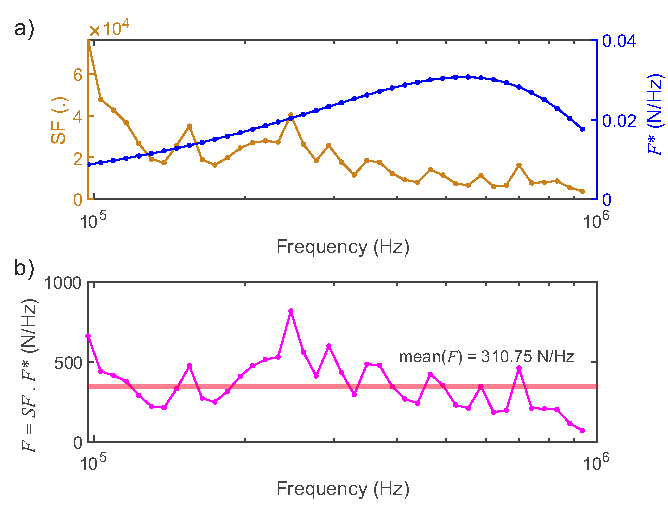
\includegraphics[scale= 1]{FIG8.pdf} 
\caption{\textbf{(a)}  }
	\label{fig8} 
\end{figure}


\begin{figure}[ht]
     	\centering
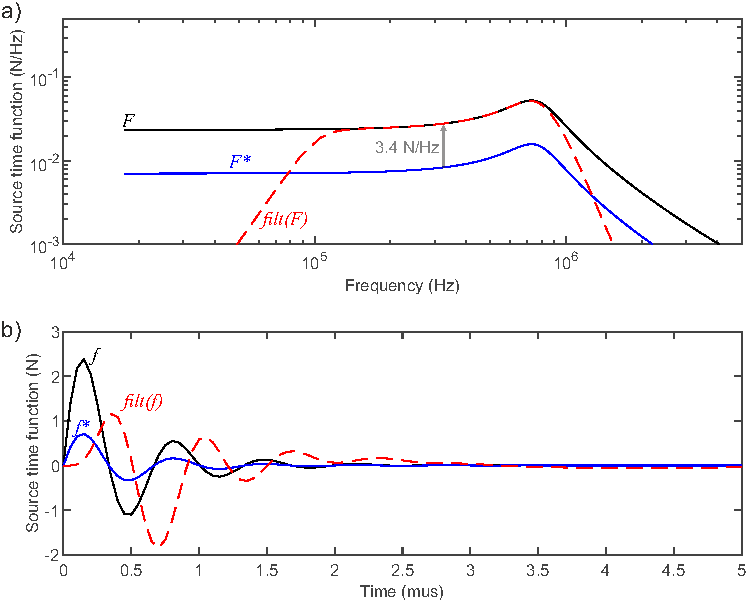
\includegraphics[scale= 1]{FIG9.pdf} 
\caption{\textbf{(a)}  }
	\label{fig9} 
\end{figure}

\begin{figure}[ht]
     	\centering
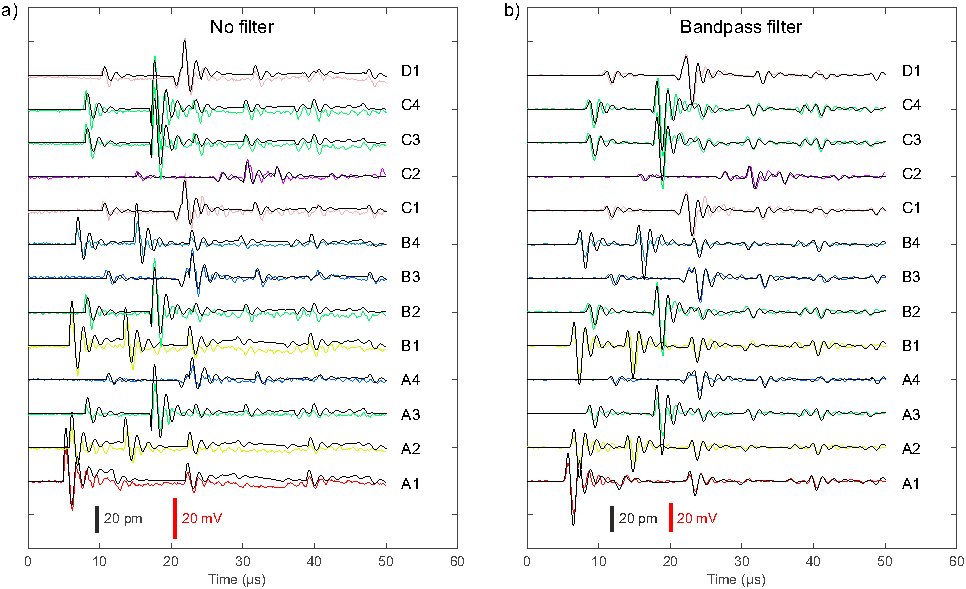
\includegraphics[scale= 1]{FIG10.pdf} 
\caption{\textbf{(a)}  }
	\label{fig10} 
\end{figure}



\section*{Acknowledgement}






\bibliographystyle{elsarticle-harv} 
\bibliography{Source_reconstruction}

\end{document}
\endinput
